% question 4
\qs{}{
    How many subjects does Taylor Sheesh have?
}

Create a view for Taylor's information. This view's \texttt{stud\_id} serves as the filter for the query in the enrollment table.
\vspace{\baselineskip}

\sol{}
\noindent\line(1, 0){0.89\linewidth}
\begin{verbatim}
create view sheesh as
select * from student where stud_fname = "Taylor" and stud_lname = "Sheesh";

select count(crs_id) as "Taylor's Subjects" from enrollment en where
en.stud_id = (select stud_id from sheesh);
\end{verbatim}
\noindent\line(1, 0){\linewidth}

\begin{figure}[H]
    \centering
    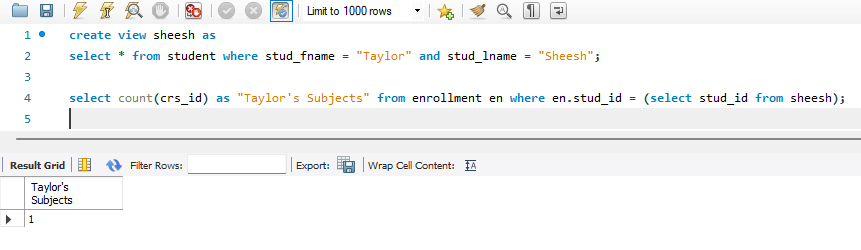
\includegraphics[width=0.7\linewidth]{images/q4.png}
    \caption{Question 4 Query and Output}
\end{figure}
